\chapter{Implementation}\label{chapter:implementation}

This project has been implemented as an MITK plugin. MITK, the Medical Imaging Interaction Toolkit, is a free open-source software system for the development of interactive medical image processing software. It combines ITK (for image processing) and VTK (for visualization) together with a basic application, the MITK Workbench, that can be extended with plugins. The UI for the plugin uses Qt, a cross-platform UI framework.

\begin{figure}[H]
  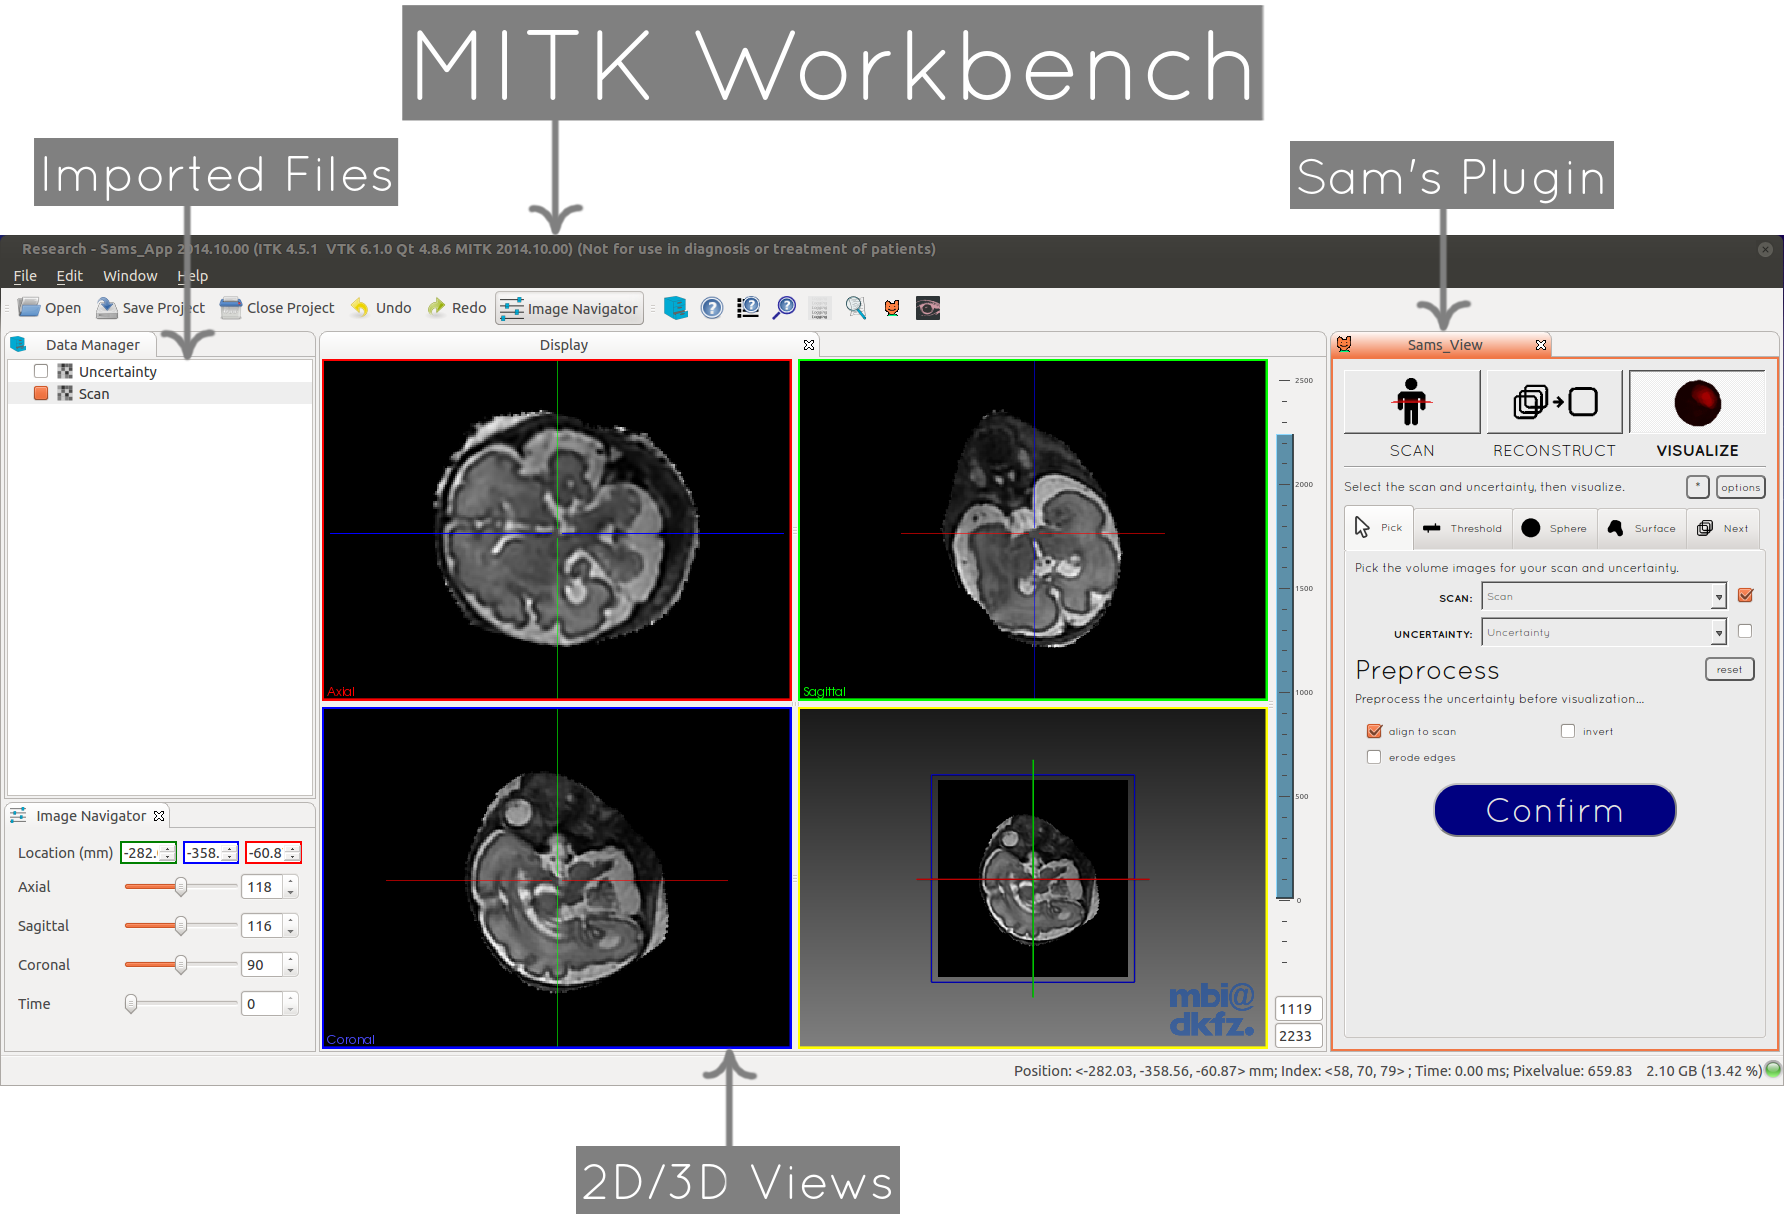
\includegraphics[width=\textwidth]{images/tool/mitk.png}
  \caption{MITK Workbench + Plugin}\label{fig:mitkoverview}
\end{figure}

The plugin developed incorporates features from all three stages of the reconstruction pipeline: scan, reconstruct, visualize. Each stage has a separate page that can be selected from the top of the plugin window. The rest of this chapter explains the features available in each.

\clearpage
\section{Scan Simulation}\label{implementation:scan_simulation}
The idea behind simulating a scan is that we can evaluate the performance of reconstruction algorithms if we can compare the result to a known, 'perfect', reconstruction. The focus of this part of the tool is not to evaluate the effectiveness of this approach, which is a project in its own right, but to make this simulation easier to perform and customize for future research.

\begin{wrapfigure}[23]{r}{0.4\textwidth}
  \vspace{-20pt}
  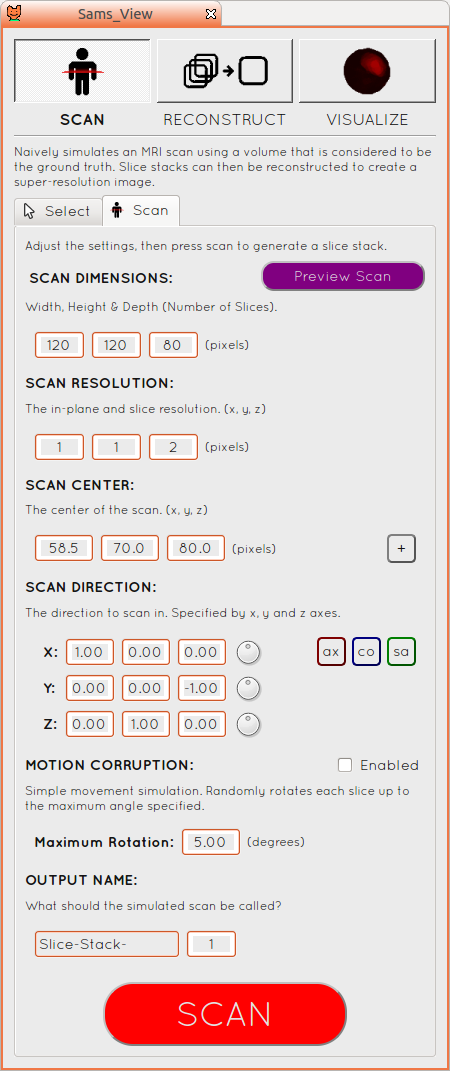
\includegraphics[width=0.4\textwidth]{images/scan_simulation/scan_settings.png}
  \caption{Controls}\label{fig:scansettings}
\end{wrapfigure}

The user has a number of controls available to tweak (figure \ref{fig:scansettings}):

\subsubsection*{Scan Dimensions}
Number of pixels in the scan (x, y, z).

\subsubsection*{Scan Resolution}
Size of each pixel (x, y, z). Measured in pixels, relative to the reconstructed scan.

\subsubsection*{Scan Center}
The center point of the scan (x, y, z). This can be set to the center of the volume or adjusted manually.

\subsubsection*{Scan Direction}
The direction of the scan. The x and y directions specify the in-plane vectors and the z direction specifies the through plane or slice vector. The standard axial, coronal and sagittal scans are available and the direction can also be rotated about each axis using the dials.

\subsubsection*{Motion Corruption}
Simple motion corruption can be enabled. Motion occurs in between slices. The slice is rotated a random amount of degrees (up to the maximum specified) about a random axis.

\clearpage
A preview to illustrate the scan area is overlayed on a volume rendering of the 'perfect' reconstruction. Whenever any control changes this preview updates. Figure \ref{fig:scansimulationexample} shows an example preview and corresponding scan. The scan being simulated is axial (y-axis) and has been simulated with up to 5 degrees of motion corruption. Individual slices are perfectly scanned, however when viewed from the side successive slices don't line up due to movement.

\begin{figure}[H]
  \centering
  \begin{subfigure}[b]{0.5\textwidth}
    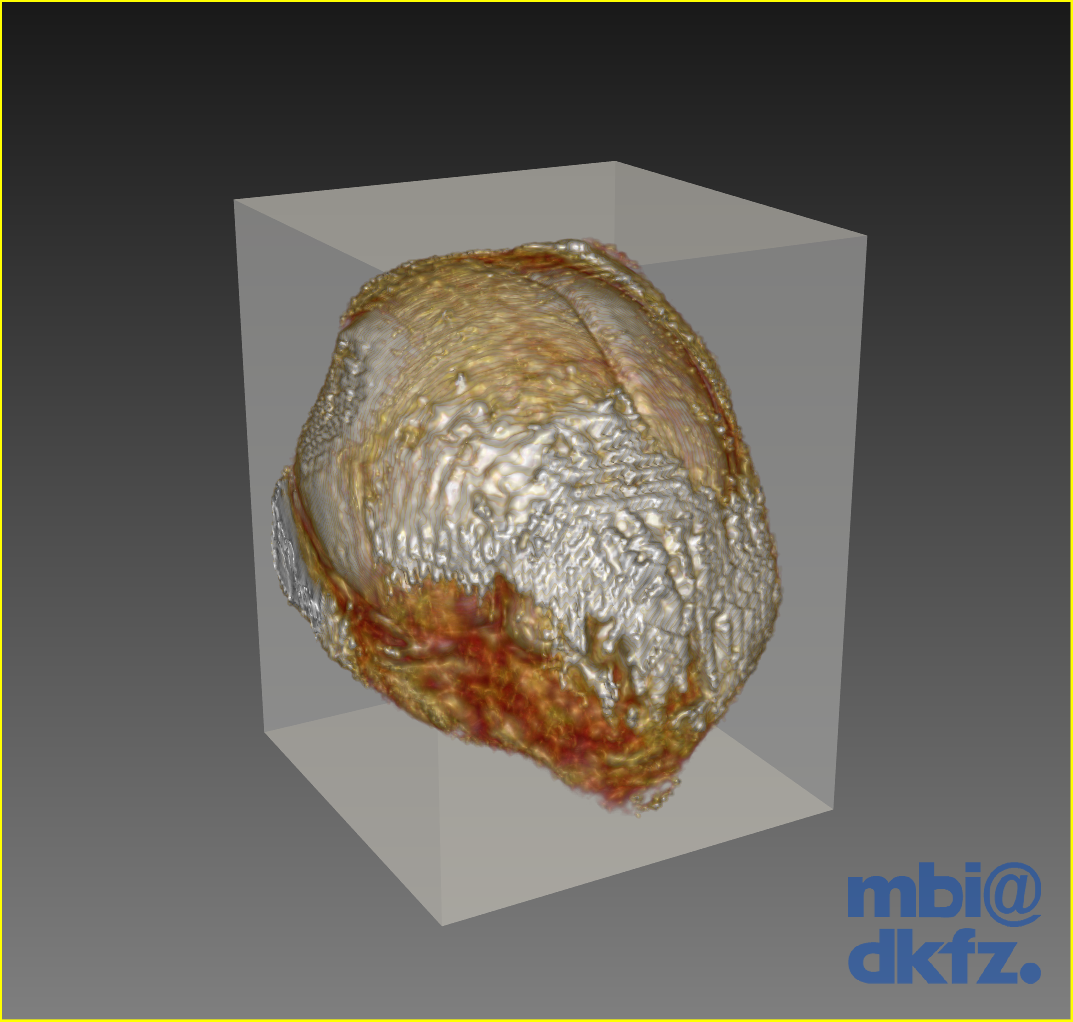
\includegraphics[width=\textwidth]{images/scan_simulation/scan_axial_preview.png}
    \caption{Scan Preview}\label{fig:scansimulationpreview}
  \end{subfigure}%
  ~ %add desired spacing between images, e. g. ~, \quad, \qquad, \hfill etc.
    %(or a blank line to force the subfigure onto a new line)
  \begin{subfigure}[b]{0.5\textwidth}
    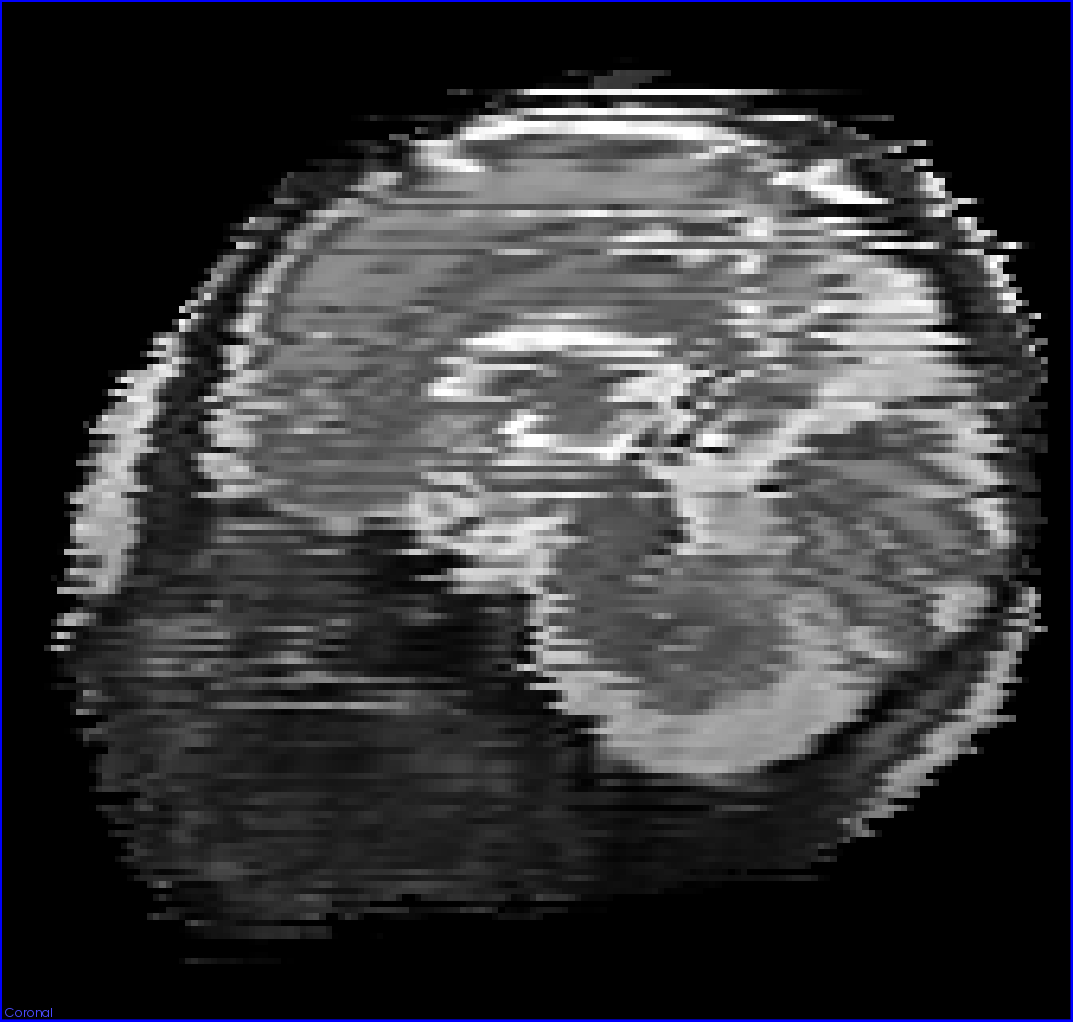
\includegraphics[width=\textwidth]{images/scan_simulation/scan_axial_result.png}
    \caption{Side (Sagittal) View of Simulation}\label{fig:scansimulationresult}
  \end{subfigure}
  \caption{Example Scan Simulation}\label{fig:scansimulationexample}
\end{figure}

\clearpage
\section{Reconstruction}\label{implementation:reconstruction}
This part of the tool provides an interface to the fast GPU reconstruction code developed in \cite{uncertaintysvd}. Currently the reconstruction code has to be compiled separately but once the plugin knows where the binary is it can make calls to it. Figure \ref{fig:reconstruction_overview} shows the inputs and outputs of the reconstruction algorithm. A dotted line indicates that the input is optional.

\begin{figure}[h]
  \centering
  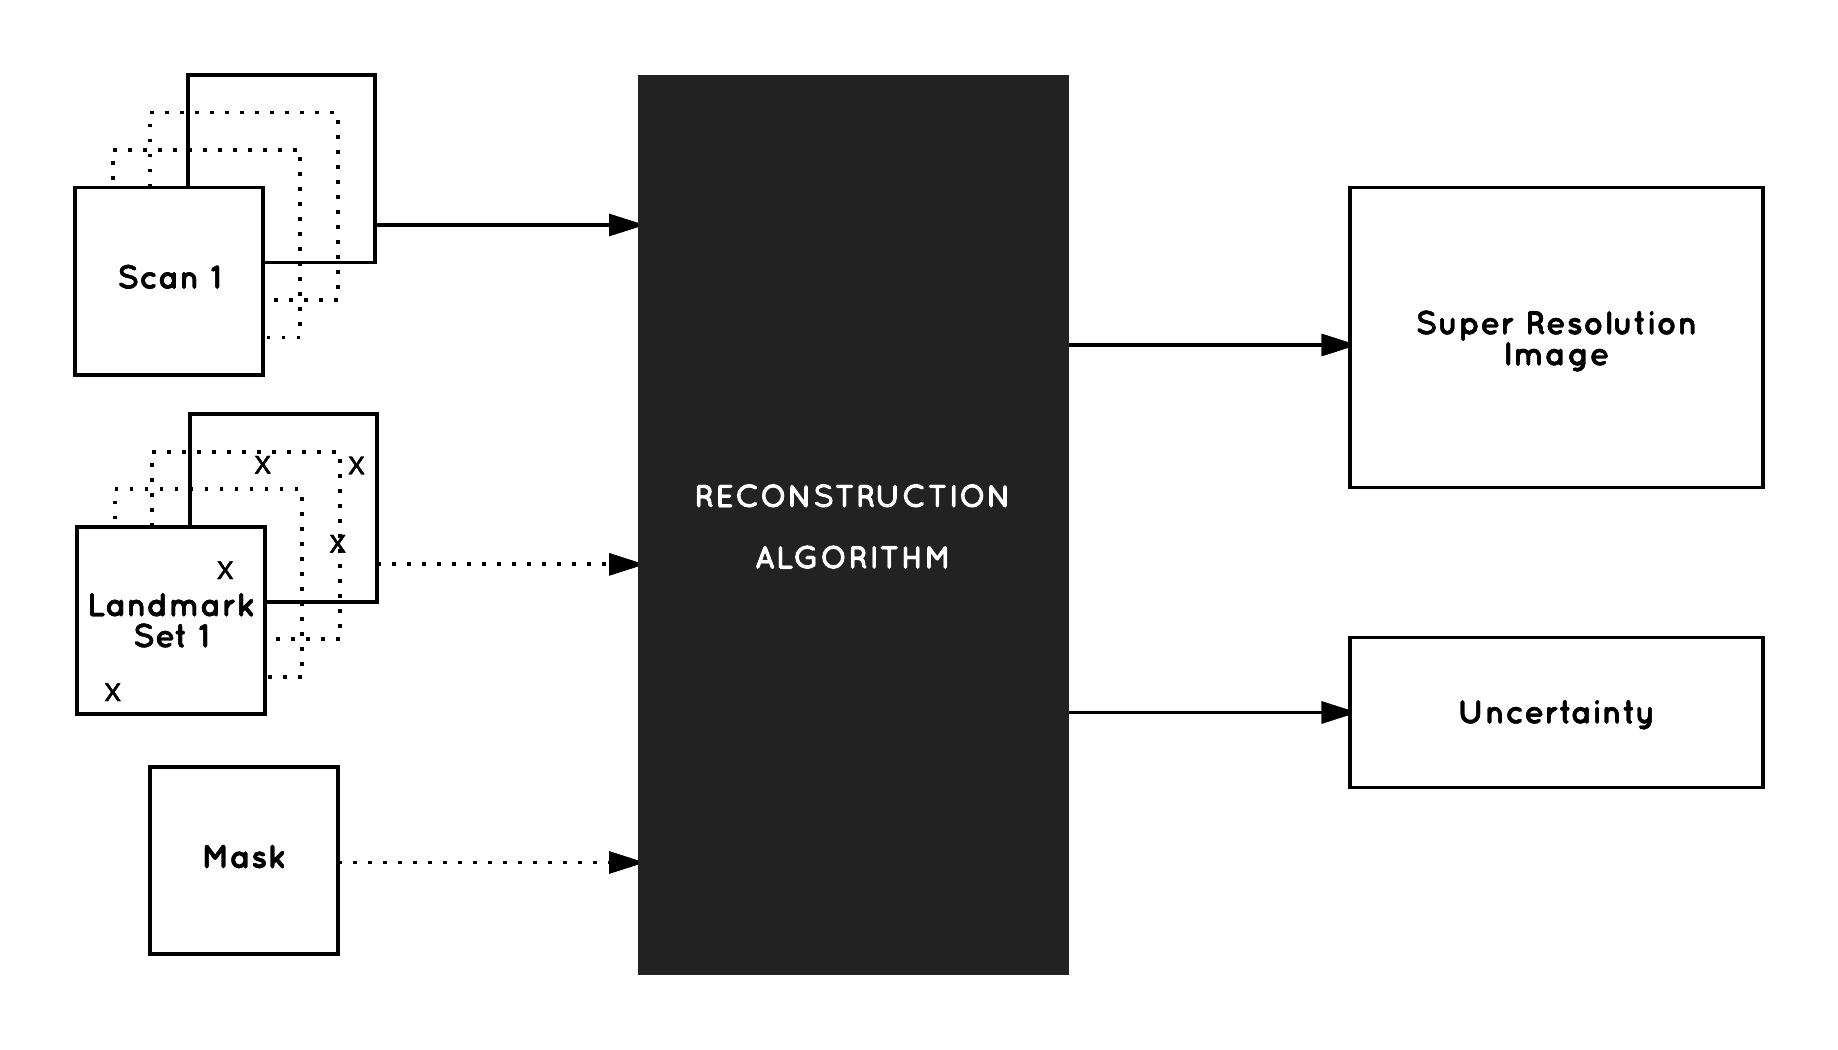
\includegraphics[width=0.8\textwidth]{images/reconstruction_overview.png}
  \caption{Reconstruction Overview}
  \label{fig:reconstruction_overview}
\end{figure}

The SVR process takes in a set of slice stacks (scans), a set of landmarks (optional) and mask (optional) and outputs the reconstructed MRI volume and uncertainty. The mask is used to ignore areas that are not of interest; for example when doing a fetal scan a mask can be created to ignore surrounding areas like the womb and amniotic fluid. A set of landmarks can be provided for each slice stack which are used by the reconstruction algorithm to help with registration.

Figure \ref{fig:reconstructionlandmarks} shows the optional landmarking stage. The landmarks are placed in the order listed and the status of each is shown by the indicator to the left of the landmark name. Grey indicates that the landmark has yet to be placed, purple shows the next landmark to be found and green indicates it has already been placed. 

Landmarks are placed by pressing "shift + left click" in the 2D view and can be dragged around once down, or deleted by pressing the black button next to the landmark name. Clicking the indicator of landmark that has been placed will jump to and select it in the 2D view. The currently selected landmark is shown in red in the 2D view and marked by an arrow in the indicator.

\begin{figure}[H]
  \centering
  \begin{subfigure}[b]{0.559\textwidth}
    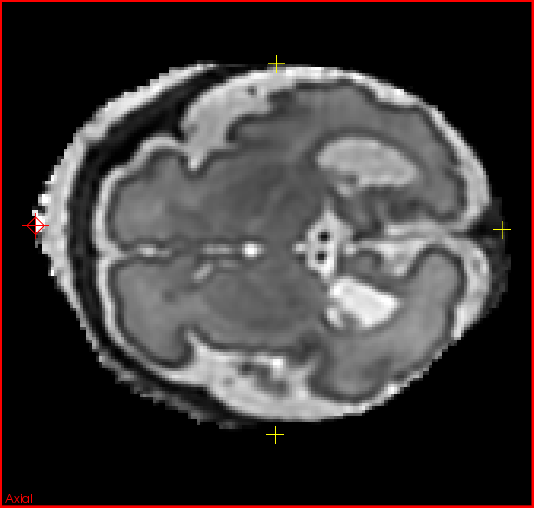
\includegraphics[width=\textwidth]{images/reconstruction/axial.png}
    \caption*{Axial}
    \label{fig:reconstructionaxial}
  \end{subfigure}%
    %add desired spacing between images, e. g. ~, \quad, \qquad, \hfill etc.
    %(or a blank line to force the subfigure onto a new line)
  \begin{subfigure}[b]{0.441\textwidth}
    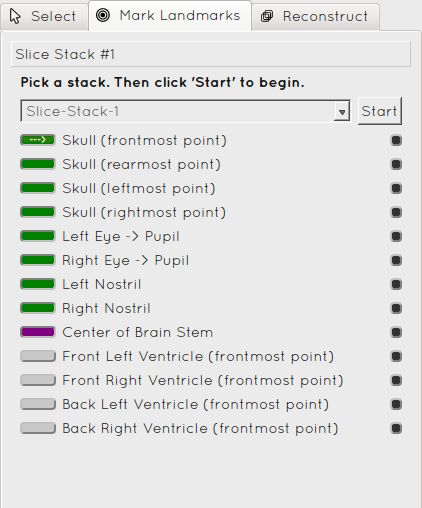
\includegraphics[width=\textwidth]{images/reconstruction/controls.png}
    \caption*{Controls}
    \label{fig:reconstructioncontrols}
  \end{subfigure}
  \caption{Placing Landmarks on Slice Stacks.}\label{fig:reconstructionlandmarks}
\end{figure}

\clearpage
\section{Visualizations}\label{implementation:visualizations}
To visualize the uncertainty the scan volume and uncertainty volume first have to be chosen. Then the uncertainty is pre-processed; in all cases the uncertainty is normalized to be within the range [0-1] and then optionally the uncertainty can be aligned to the scan, inverted and eroded.

\subsubsection*{Normalize}
The uncertainty is linearly scaled so each value is between 0 and 1.\\(Uses $RescaleIntensityImageFilter$ from ITK)

\begin{verbatim}
  0 - no information (high uncertainty - worst)
  1 - maximum information (low uncertainty - best)
\end{verbatim}

\subsubsection*{Align to Scan}
\begin{wrapfigure}[14]{r}{0.4\textwidth}
  \vspace{-20pt}
  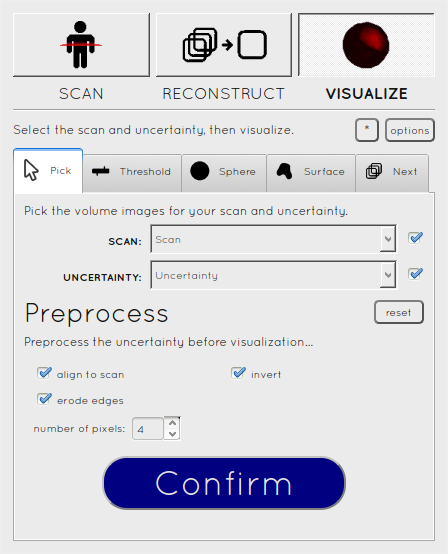
\includegraphics[width=0.4\textwidth]{images/pre-processing.png}
  \caption{Pre-processing}\label{fig:pre-processing_settings}
\end{wrapfigure}

This ensures that the scan and uncertainty occupy the same point in space. If the uncertainty has no location information (image to world matrix) then the image to world matrix of the scan is applied to it. This feature was mainly useful for aligning artificial uncertainties to a scan for testing.

\subsubsection*{Invert}
If the uncertainty volume has been saved the other way round (i.e. low is good and high is bad) then this will invert it to be compatible with the plugin.\\(Uses $InvertIntensityImageFilter$ from ITK)

\subsubsection*{Erosion}
The optional erosion step removes the uncertainty values at the edge of the reconstruction. The edges often have a much higher uncertainty either because there are fewer slices to use or the mask cuts off the data required. Removing this edge helps the visualization to focus on the core of the volume. The amount of erosion is specified as a number of pixels.\\(Uses the following ITK filters: $BinaryThresholdImageFilter$ (to threshold background), $GrayscaleDilateImageFilter$ (to grow) and $MaskImageFilter$ (to remove edge). See \ref{method:pre-processing} for details.)

\clearpage
\subsection{Thresholding}\label{implementation:thresholding}
The idea behind thresholding is to isolate areas in the reconstructed image that are within a particular range of uncertainty. 

\begin{wrapfigure}[18]{r}{0.4\textwidth}
  \vspace{-20pt}
  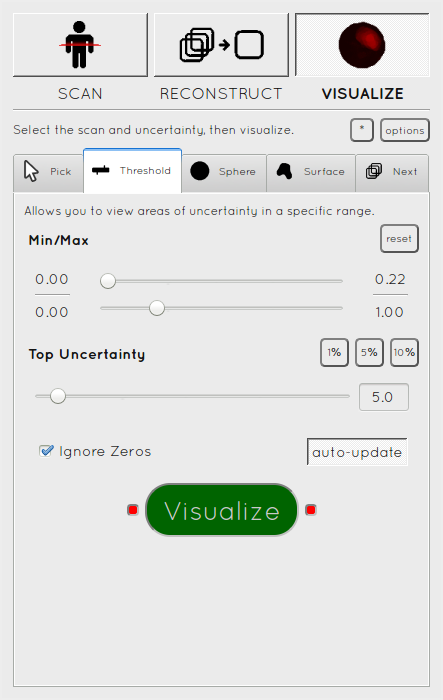
\includegraphics[width=0.4\textwidth]{images/tool/2_thresholding.png}
  \caption{Controls}\label{fig:threshold_settings}
\end{wrapfigure}

Figure \ref{fig:threshold_settings} shows the controls available to the user. The top two sliders allow the user to explicitly specify a range, like [0.2-0.5] and the bottom slider computes the bounds to isolate the worst x$\%$. The worst 5$\%$ has been selected, which has been computed to lie within the range [0.0-0.22].

'Ignore Zeros' is ticked which means the background, which has value 0.0, is not displayed even if it is within the range selected. The auto-update toggle box decides whether changes to the controls immediately update the visualization.

Figure \ref{fig:threshold_settings_result} illustrates the result.\\\\\\

\begin{figure}[H]
  \centering
  \begin{subfigure}[b]{0.4\textwidth}
    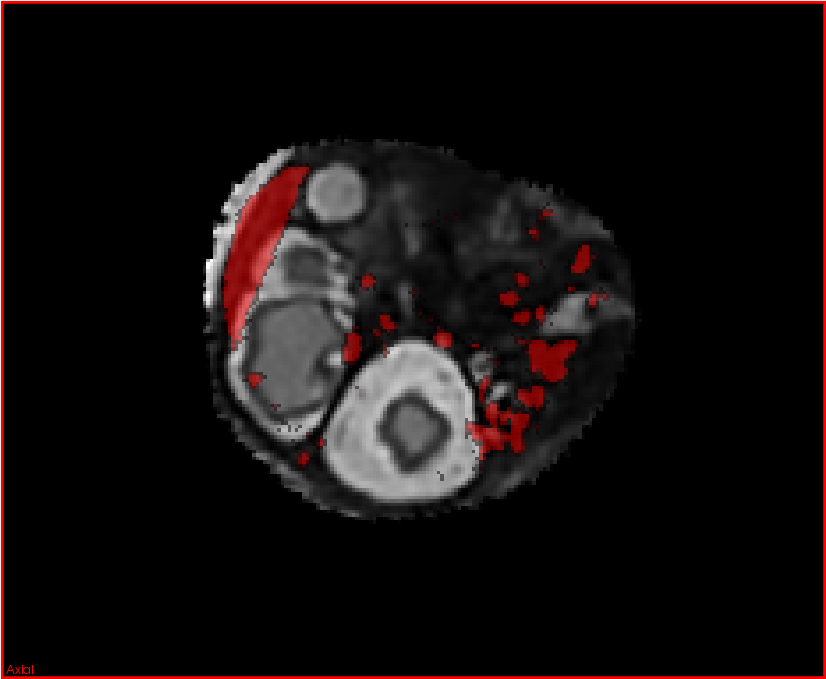
\includegraphics[width=\textwidth]{images/thresholding/thresholding_2d.png}
    \caption{2D Thresholding}\label{fig:threshold_2d}
  \end{subfigure}%
  ~ %add desired spacing between images, e. g. ~, \quad, \qquad, \hfill etc.
    %(or a blank line to force the subfigure onto a new line)
  \begin{subfigure}[b]{0.4\textwidth}
    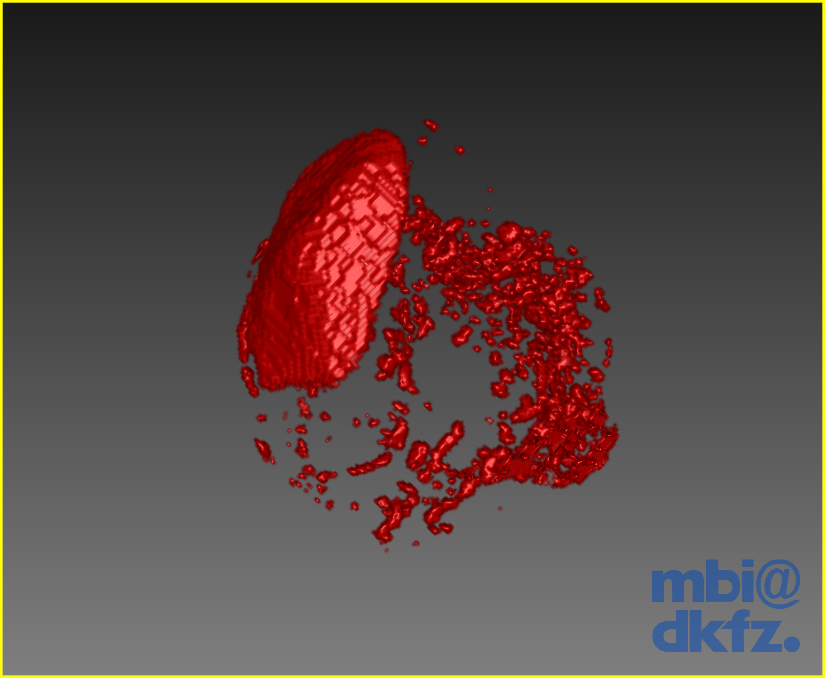
\includegraphics[width=\textwidth]{images/thresholding/thresholding_3d.png}
    \caption{3D Thresholding}\label{fig:threshold_3d}
  \end{subfigure}
  \caption{Worst 5$\%$ of Uncertainty}\label{fig:threshold_settings_result}
\end{figure}

(Uses the following ITK filters: $BinaryThresholdImageFilter$ (to threshold) and $ImageToHistogramFilter$ (to build a histogram). See \ref{method:thresholding} for details.)

\clearpage
\subsection{Sphere}\label{implementation:sphere}
The idea behind both the uncertainty sphere and uncertainty surface visualizations is to project the uncertainty, which is a 3D volume, onto a surface model, which is essentially 2D. This gives the viewer an overview of the uncertainty without having to go through each area, slice by slice.

\begin{wrapfigure}[17]{r}{0.4\textwidth}
  \vspace{-20pt}
  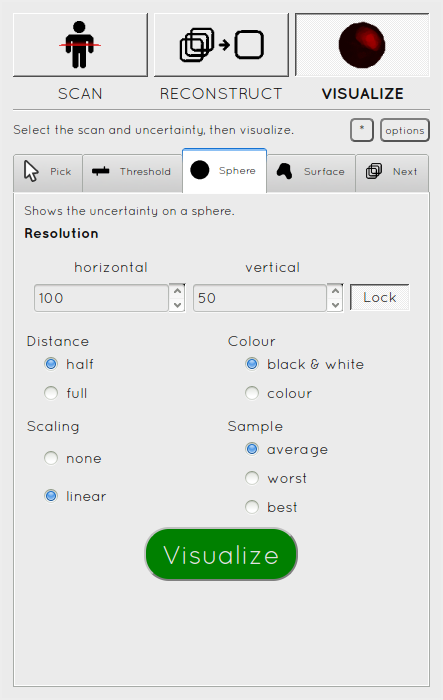
\includegraphics[width=0.4\textwidth]{images/tool/3_sphere.png}
  \caption{Controls}\label{fig:sphere_settings}
\end{wrapfigure}

The sphere is designed to be a generic visualization that can work with any scan, regardless of the target. Figure \ref{fig:sphere_settings} shows the control the user has over the visualization and figure \ref{fig:sphere_settings_result} shows the resulting visualization.

\subsubsection{Resolution}
This changes how many points are used to represent the sphere. The more points used the sharper the image, but the longer the processing takes.

\subsubsection{Distance}
This alters how far into the volume to sample. Half means that the uncertainty is sampled until the center and full means it is sampled until the edge of the image. This option is more useful in the next visualization as with the sphere full sampling generally means that opposite points have identical values.

\subsubsection{Colour}
This swaps between a black and white and a black and red visualization.

\subsubsection{Scaling}
This scales the resulting uncertainty values to make better use of the colours available. With no scaling the uncertainty values are often roughly the same everywhere and end up looking largely indistinguishable; to fix this the outputted uncertainty range can be linearly mapped to make better use of the available colours.

\subsubsection{Sample}
By default the value shown on the surface is the average of all the points along the ray. This can be altered to show the worst or best value.

\clearpage
\subsection{Surface}\label{implementation:surface}
The uncertainty surface uses a similar approach to the uncertainty sphere however uncertainty is mapped to a surface representation of the organ being scanned.

\begin{wrapfigure}[18]{r}{0.4\textwidth}
  \vspace{-20pt}
  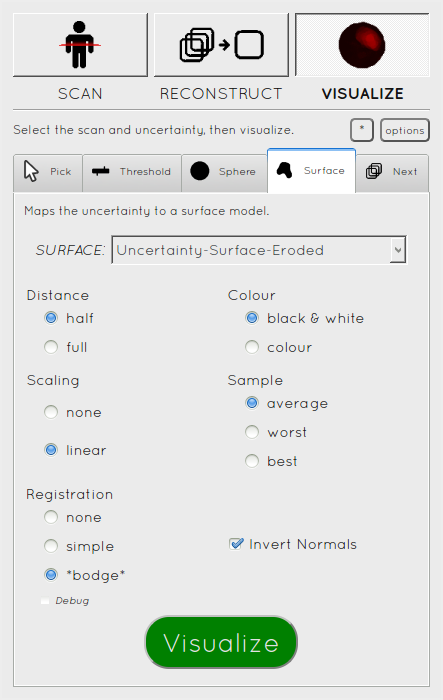
\includegraphics[width=0.4\textwidth]{images/tool/4_surface.png}
  \caption{Controls}\label{fig:surface_settings}
\end{wrapfigure}

Figure \ref{fig:surface_settings} shows the controls, which are largely the same as the sphere with three exceptions. Figure \ref{fig:surface_settings_result} shows the result.

\subsubsection{Surface}
This allows the user to pick the surface to map the uncertainty to.

\subsubsection{Registration}
This decides how the surface is aligned to the uncertainty volume. None assumes that they are already aligned. Simple finds the bounding box of the surface and maps it to the bounding box of the volume. *bodge* is just used in development. Debug marks the points that each surface point registers to on the uncertainty so the registration can be visually inspected.

\subsubsection{Invert Normals}
Inverts the normals stored at each point on the surface. Use when normals point outwards.

\begin{figure}[H]
  \centering
  \begin{subfigure}[b]{0.4\textwidth}
    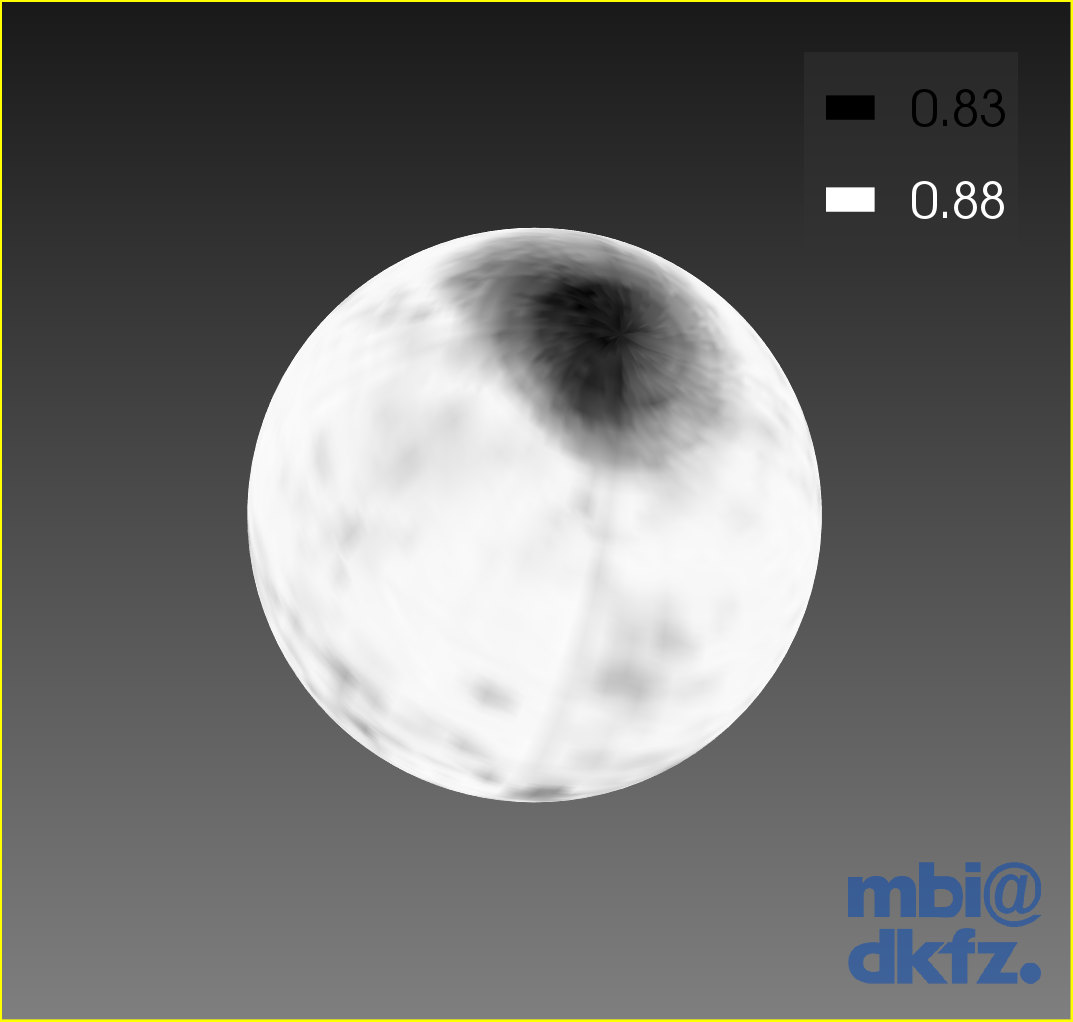
\includegraphics[width=\textwidth]{images/surface/sphere_average.png}
    \caption{Sphere}\label{fig:sphere_settings_result}
  \end{subfigure}%
  ~ %add desired spacing between images, e. g. ~, \quad, \qquad, \hfill etc.
    %(or a blank line to force the subfigure onto a new line)
  \begin{subfigure}[b]{0.4\textwidth}
    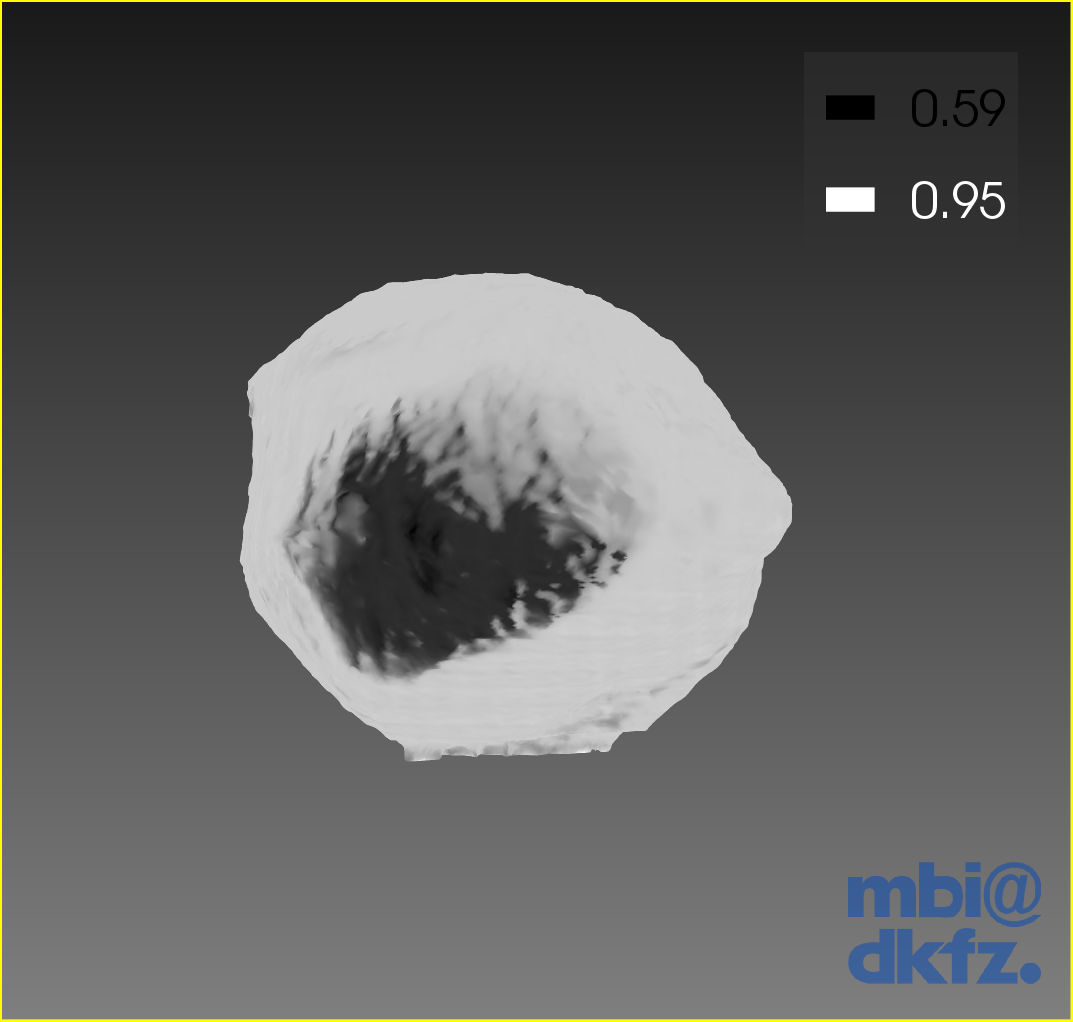
\includegraphics[width=\textwidth]{images/surface/surface_average.png}
    \caption{Surface}\label{fig:surface_settings_result}
  \end{subfigure}
  \caption{Surface Visualizations}\label{fig:surface_settings_result}
\end{figure}

\clearpage
\subsection{Next Scan Plane}\label{implementation:next_scan_plane}
The idea behind this visualization is based on research\cite{uncertaintysvd} which uses SVD to find the optimum position and direction to scan next given the current uncertainty. With this knowledge the scanning process can continually target areas of uncertainty to optimize the quality of the reconstruction.

\begin{wrapfigure}[18]{r}{0.4\textwidth}
  \vspace{-20pt}
  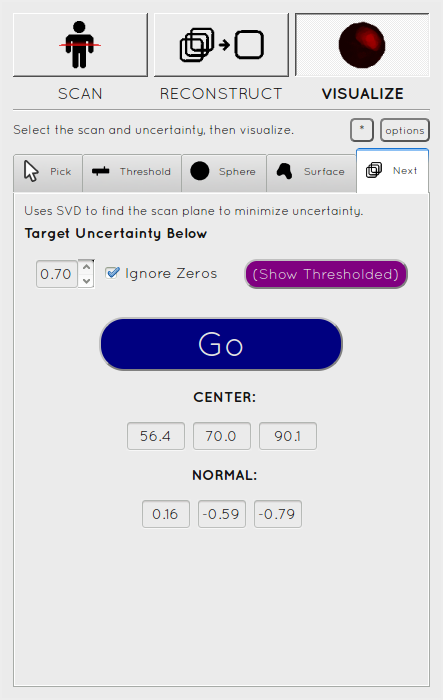
\includegraphics[width=0.4\textwidth]{images/tool/5_next_scan_plane.png}
  \caption{Controls}\label{fig:next_scan_plane_settings}
\end{wrapfigure}

This visualization is designed to communicate the next best scan to the radiographer in a way that also provides some context as to why this is optimal. Figure \ref{fig:next_scan_plane_settings} shows the controls available.

\subsubsection{Target Uncertainty}
The user chooses the uncertainty to target by specifying an upper threshold. This threshold can then be previewed using thresholding before the next scan is computed. The resulting scan is then visualized as a circle, which shows the central slice of the scan, and a cylinder which indicates the direction of the scan. The scan volume can also be volume rendered to illustrate where on the target the scan is.

As well as being shown visually the center and normal of the next best scan is also shown underneath the 'Go' button.

Figure \ref{fig:nextscanplane} illustrates this process.\\

\begin{figure}[H]
  \centering
  \begin{subfigure}[b]{0.32\textwidth}
    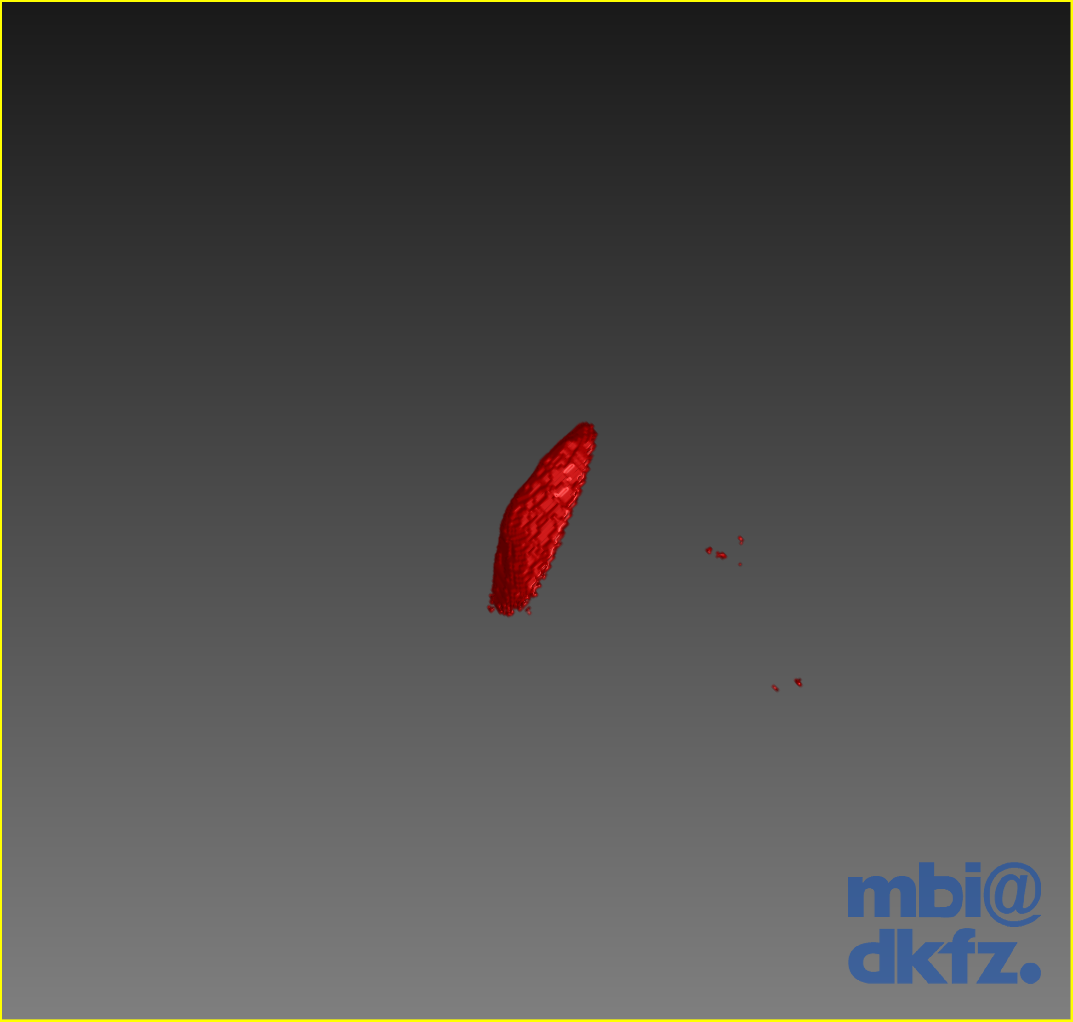
\includegraphics[width=\textwidth]{images/next_scan_plane/next_scan_plane_threshold.png}
    \caption*{Uncertainty to target.}
    \label{fig:nextscanplanethreshold}
  \end{subfigure}%
  ~ %add desired spacing between images, e. g. ~, \quad, \qquad, \hfill etc.
    %(or a blank line to force the subfigure onto a new line)
  \begin{subfigure}[b]{0.32\textwidth}
    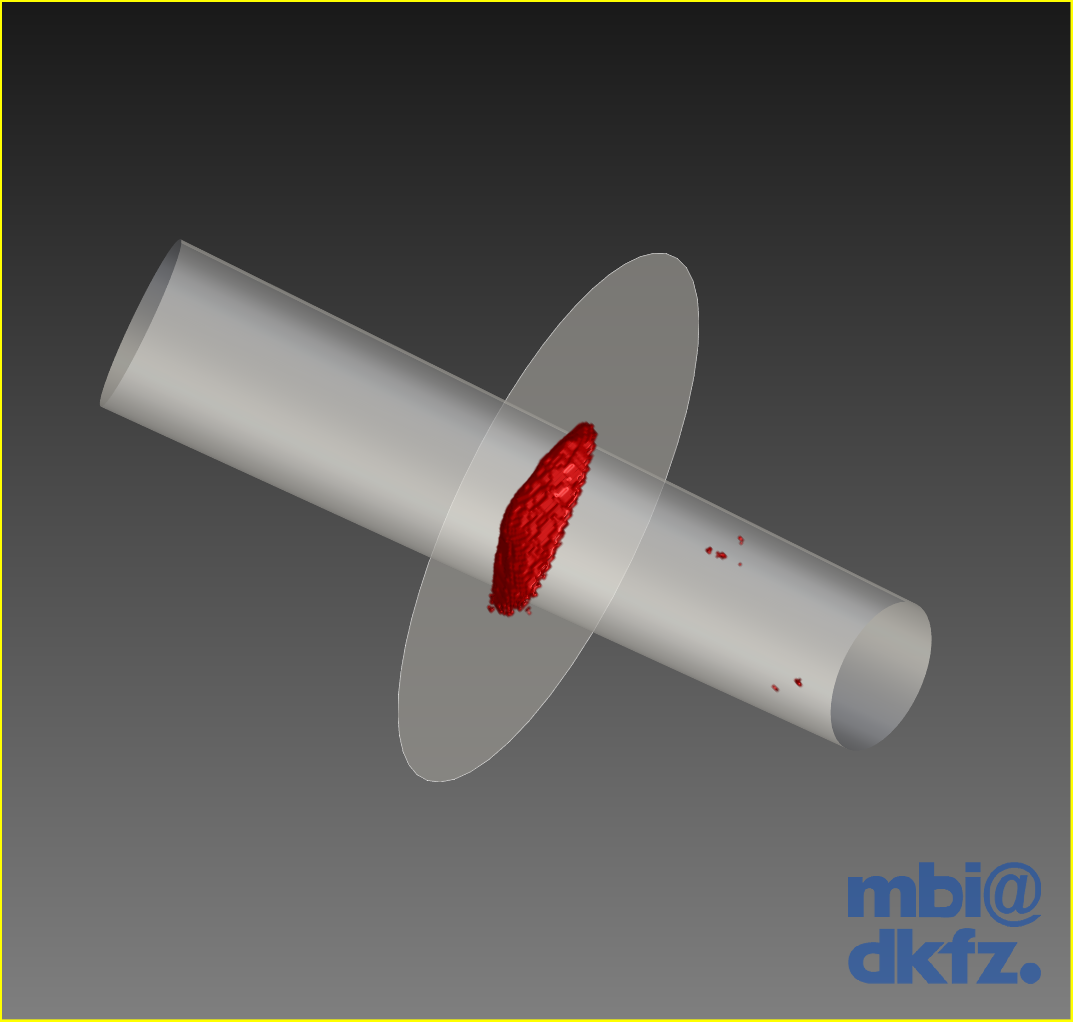
\includegraphics[width=\textwidth]{images/next_scan_plane/next_scan_plane_1.png}
    \caption*{Next scan plane.}
    \label{fig:nextscanplane1}
  \end{subfigure}%
  ~ %add desired spacing between images, e. g. ~, \quad, \qquad, \hfill etc.
    %(or a blank line to force the subfigure onto a new line)
  \begin{subfigure}[b]{0.32\textwidth}
    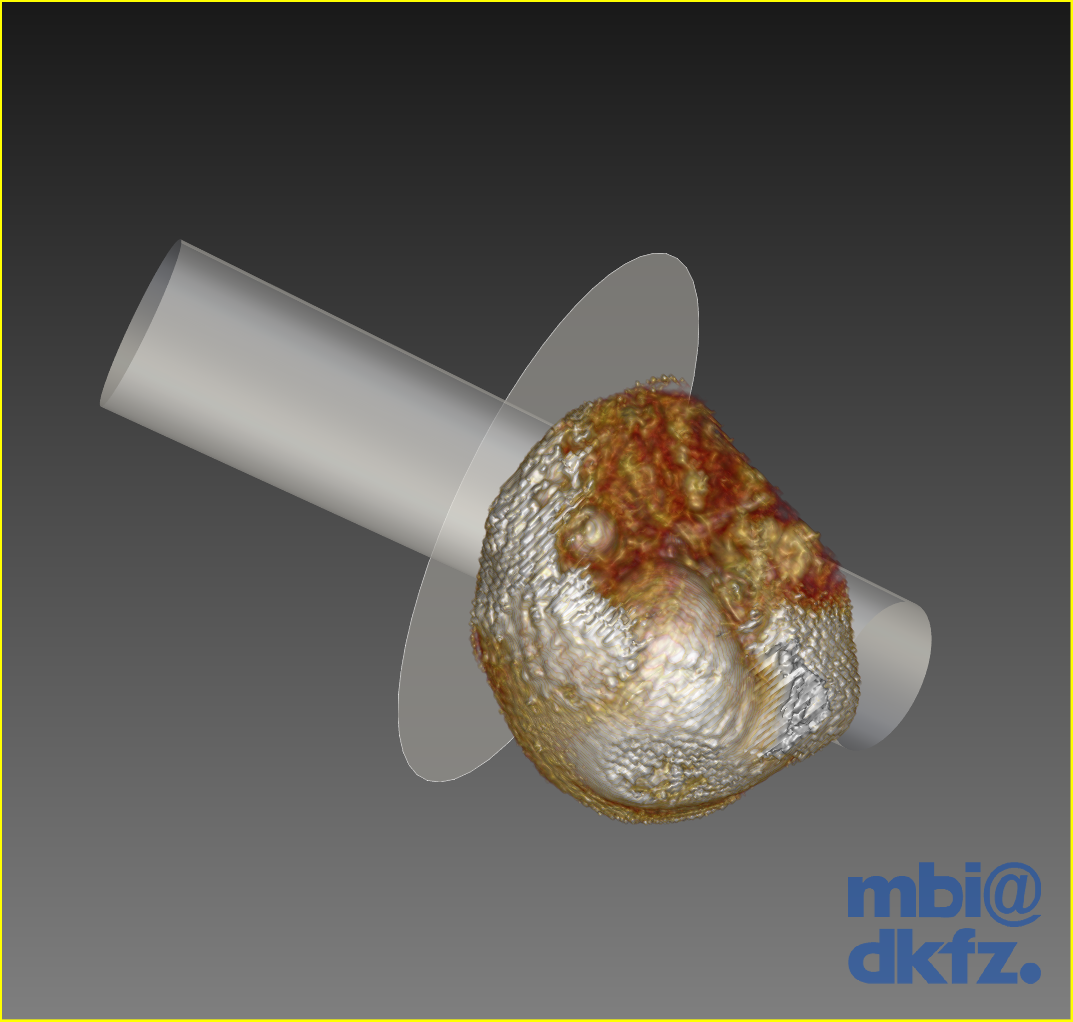
\includegraphics[width=\textwidth]{images/next_scan_plane/next_scan_plane_2.png}
    \caption*{With scan volume.}
    \label{fig:nextscanplane2}  
  \end{subfigure}
  \caption{Next scan plane process.}\label{fig:nextscanplane}
\end{figure}